\chapter{Experiments}

\section{Measure acceptance angle}
As a general verification of the system and a second verify the
alignment of the MMA on the back focal plane of the objective lens, we
imaged three fluorescent plane samples with various embedding indices.

The illumination in the sample is a disk of $\unit[30]{\mu m}$
diameter, spanning nearly the full field. Then a window of
$15\times15$ pixels was scanned over the MMA and for each position, a
camera image was captured. \figref{fig:immersion-bfp-scan} displays
the integrated intensity in each image for each of the positions on
the back focal plane.

The left diagram shows an image of the pupil of the objective. Rays in
the edges of the MMA are absorbed by the pupil aperture in the
objective and therefor dark. The next two images show the reduced
acceptance angle due to lower index embedding medium. Rays on the
border of the pupil traverse the objective but are reflected at the
coverslip--embedding interface.

\begin{figure}[!hbt]
  \centering
  \input{tirf-exp.eps_tex} 
  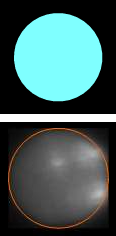
\includegraphics[height=69.56mm]{screen_mma-disk-integrate_rot}
  \caption{A fluorescent plane on a slide is embedded in oil, water or
    air. The thickness of the embedding medium is approximately
    $\unit[5]{\mu m}$. The LCoS illuminates a disk with $\unit[30]{\mu
      m}$ diameter while a $15\times 15$ window is scanned over the
    MMA. {\bf right top:} LCoS mask. {\bf right bottom:} Typical
% 200 px diameter on LCoS
% 15x15 px full diameter is D=2*(R=f*NA) f=164.5/63=2.61  NA=1.38
% D=3.6mm -> D/256*15 = 210 um
    camera image.}
  \label{fig:tirf-exp}
\end{figure}


\begin{figure}[!hbt]
  \centering
  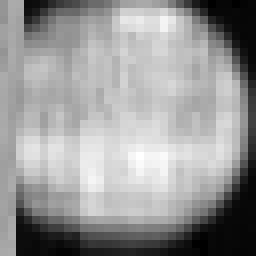
\includegraphics[width=4cm]{oil}
  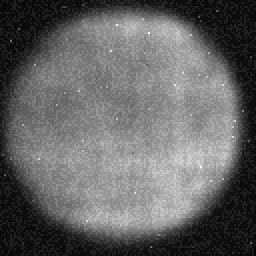
\includegraphics[width=4cm]{water}
  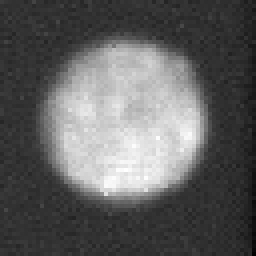
\includegraphics[width=4cm]{air}
  \caption{Integrated image intensities for different illumination
    window positions in the back focal plane. Embedding media: {\bf
      left:} Oil $n=1.52$, {\bf middle:} water $n=1.33$, {\bf right:}
    air $n=1$.  }
  \label{fig:immersion-bfp-scan}
\end{figure}
